\newpage

\section{Sample fuzzy rule}

\subsection{Turning rule}

This section will examine the implementation of the fuzzy rules that govern the saucer's ability to turn, and will use the following situation, as shown in Figure 4 to demonstrate how the \emph{turn} output rules are fired:

\begin{figure}[H]
\centering
\caption{Sample game screen}
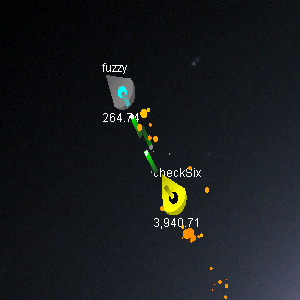
\includegraphics[scale=1]{./img/png/gameScreen.png}
\end{figure}

The yellow saucer in Figure 4 is the \emph{player}, called \emph{checkSix}, while the enemy is the grey saucer, called \emph{fuzzy}. Note that \emph{fuzzy} is controlled with the original, existing fuzzy controller supplied with the assignment. Two \emph{turn} rules are fired during this sequence:

\begin{itemize}
	\item Rule 1:
		\begin{itemize}
			\item IF (\emph{heading angle} IS front) AND (\emph{energy difference} IS winning) THEN (\emph{turn} IS 0)
		\end{itemize}	 
	\item Rule 2:
		\begin{itemize}
			\item IF (\emph{heading angle} IS left front) AND (\emph{energy difference} IS winning) THEN (\emph{turn} IS 90)
		\end{itemize}
\end{itemize}

\subsubsection{\emph{Energy difference} antecedent}

\emph{Energy difference} will be explored first, since the value is the same in both instances of Rule 1 and Rule 2 above. The \emph{energy difference} antecedent, which in this case is \emph{winning}, is demonstrated by the difference of energy between the two saucers. \emph{checkSix} has 3940.71 joules of energy remaining, while \emph{fuzzy} only has 264.74. The \emph{energy difference} is +3675.97j. Therefore, \emph{checkSix} is \emph{winning}. Figure 5 below demonstrates the firing of this antecedent, and shows that the fuzzy set value is +3675.97, while $\mu$, the membership value to the \emph{winning} fuzzy set, is 1.

\begin{figure}[H]
\centering
\caption{\emph{Energy difference} antecedent}
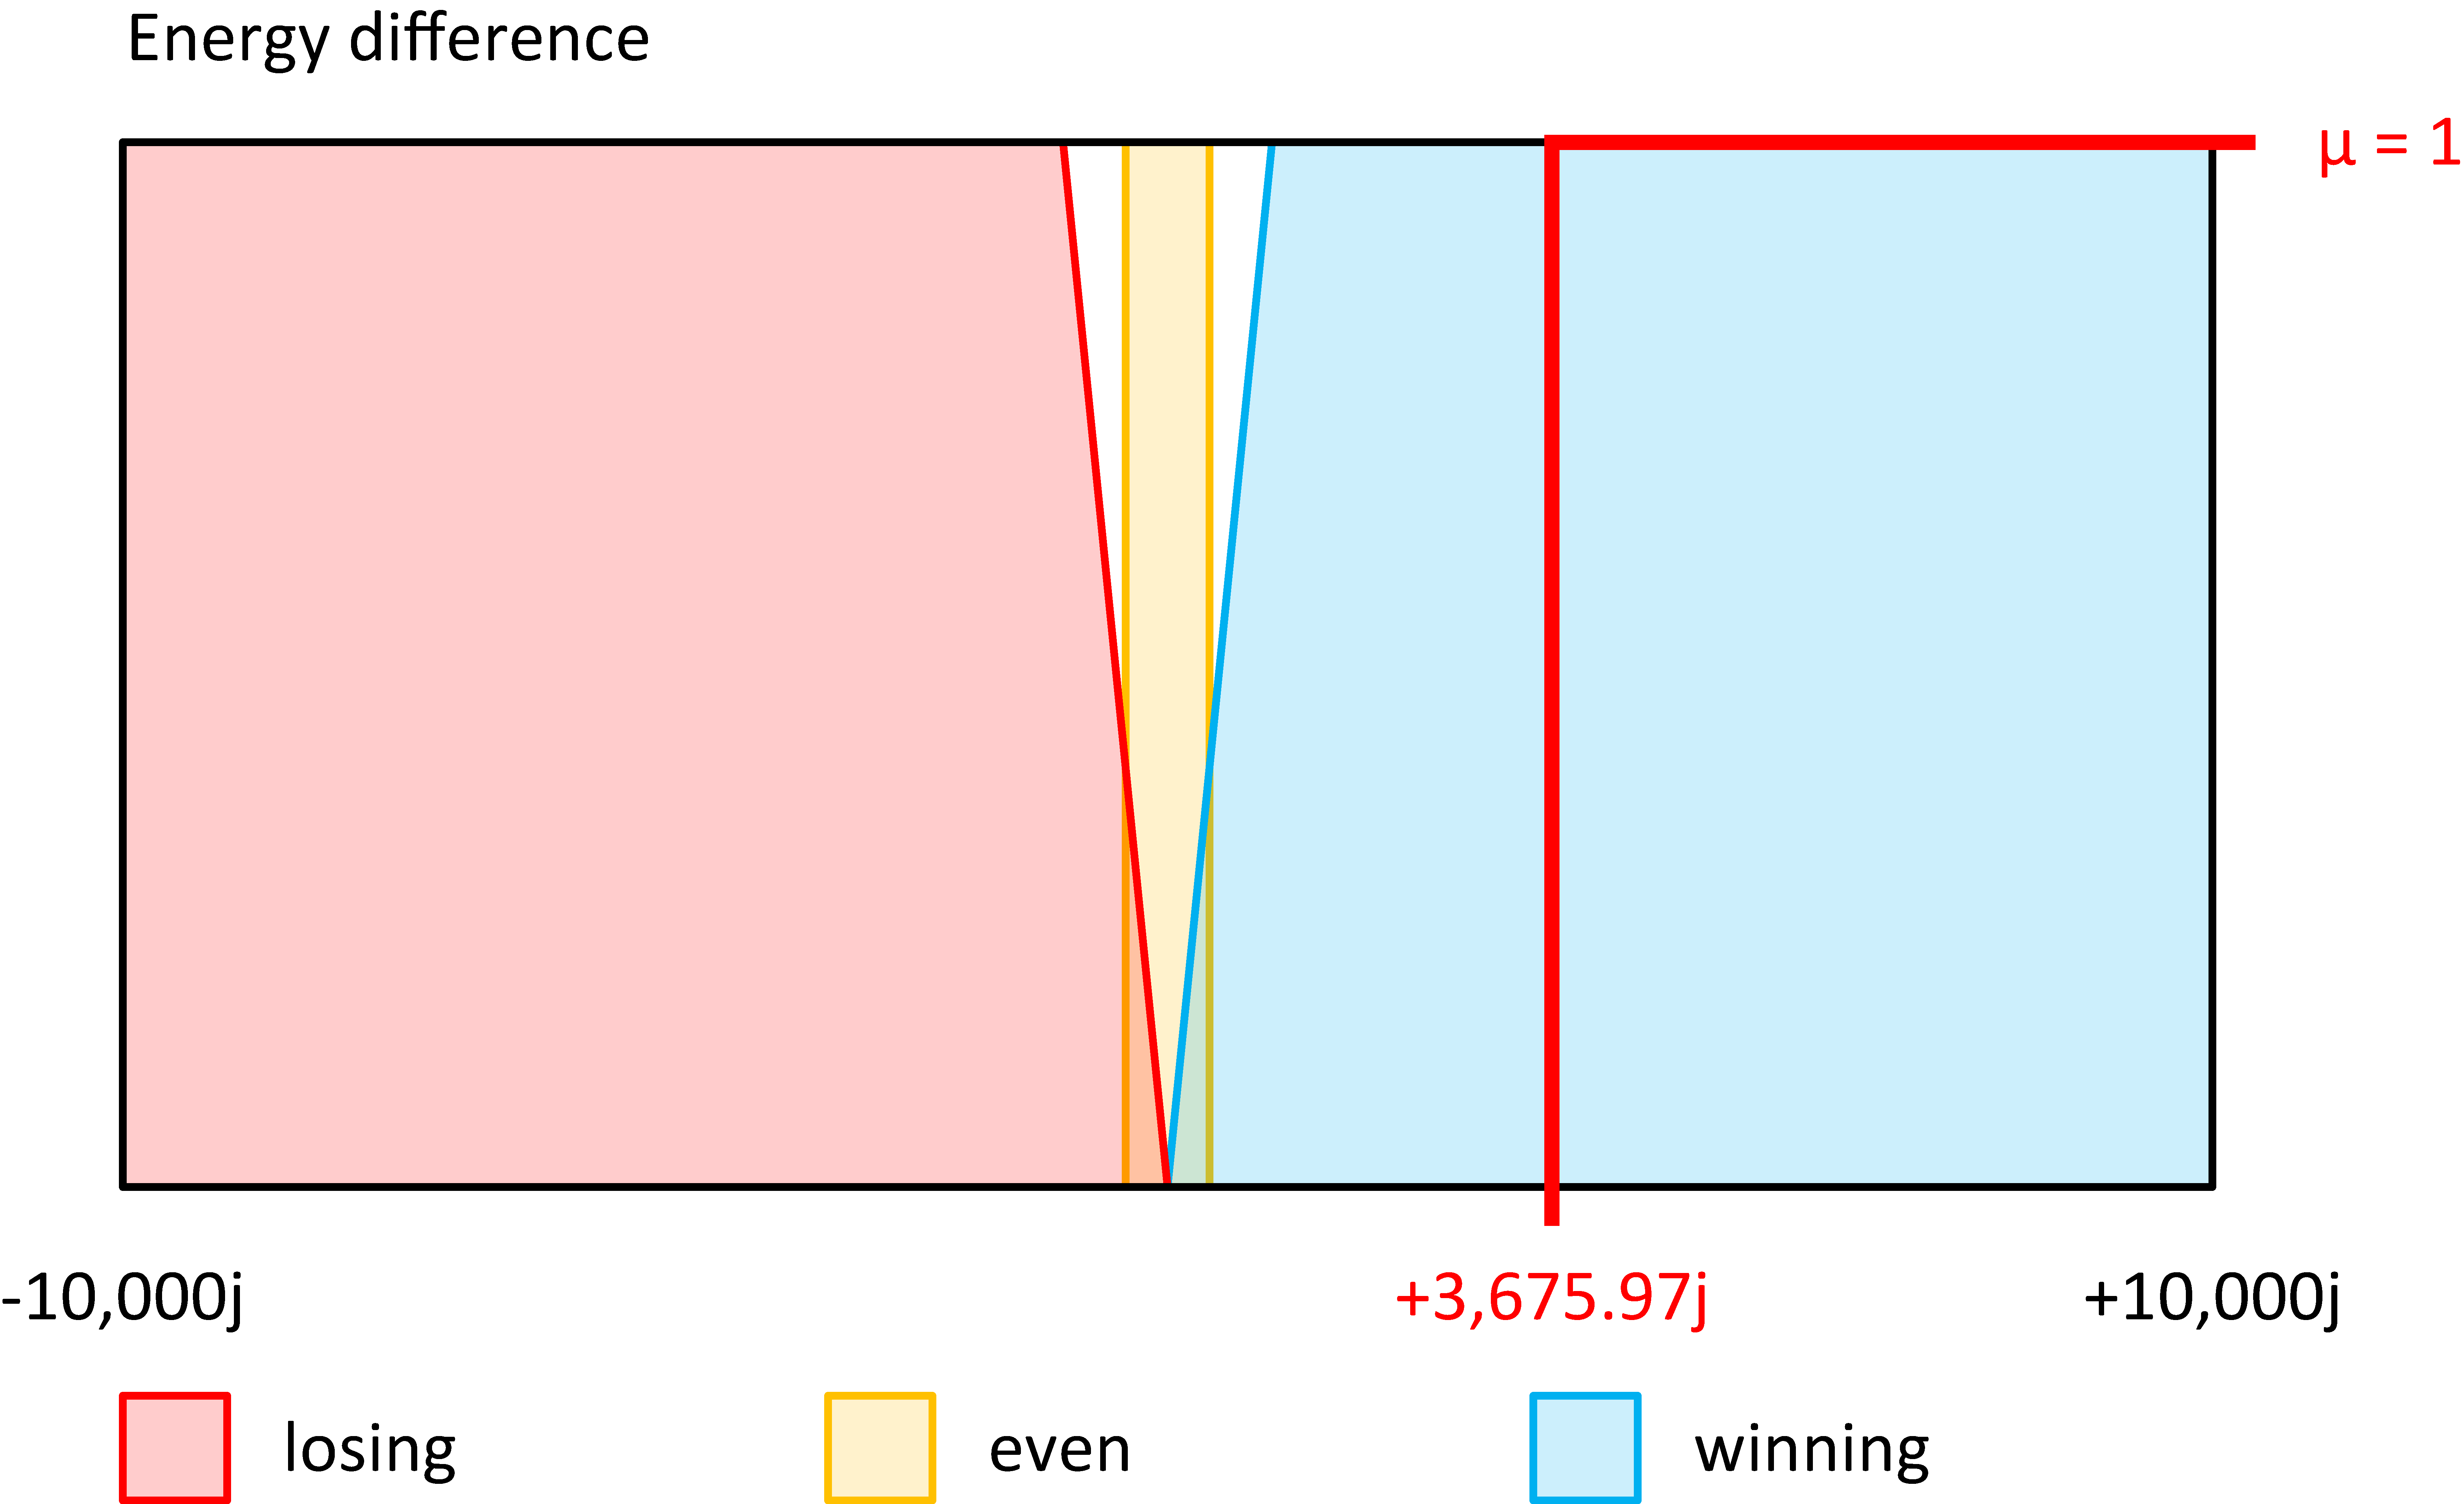
\includegraphics[scale=0.1]{./img/pdf/turnRule_energyDiff.pdf}
\end{figure}

\subsubsection{\emph{Heading angle} antecedent}

\emph{Heading angle} causes Rule 1 and Rule 2 to fire, with \emph{front} and \emph{leftFront}. This is due to the configuration of the two fuzzy sets. As seen previously in Figure 3, the \emph{leftFront} fuzzy set begins at 50\% of the \emph{front} fuzzy set range. In other words, any value higher than the median value of \emph{front} will also belong to the \emph{leftFront} set. Conversely, any value lower than the median value of \emph{front} will also belong to the \emph{rightFront} set. Figure 6 below demonstrates the firing of these two antecedents, their fuzzy set values and their $\mu$ values.

\begin{figure}[H]
\centering
\caption{\emph{Heading angle} antecedent}
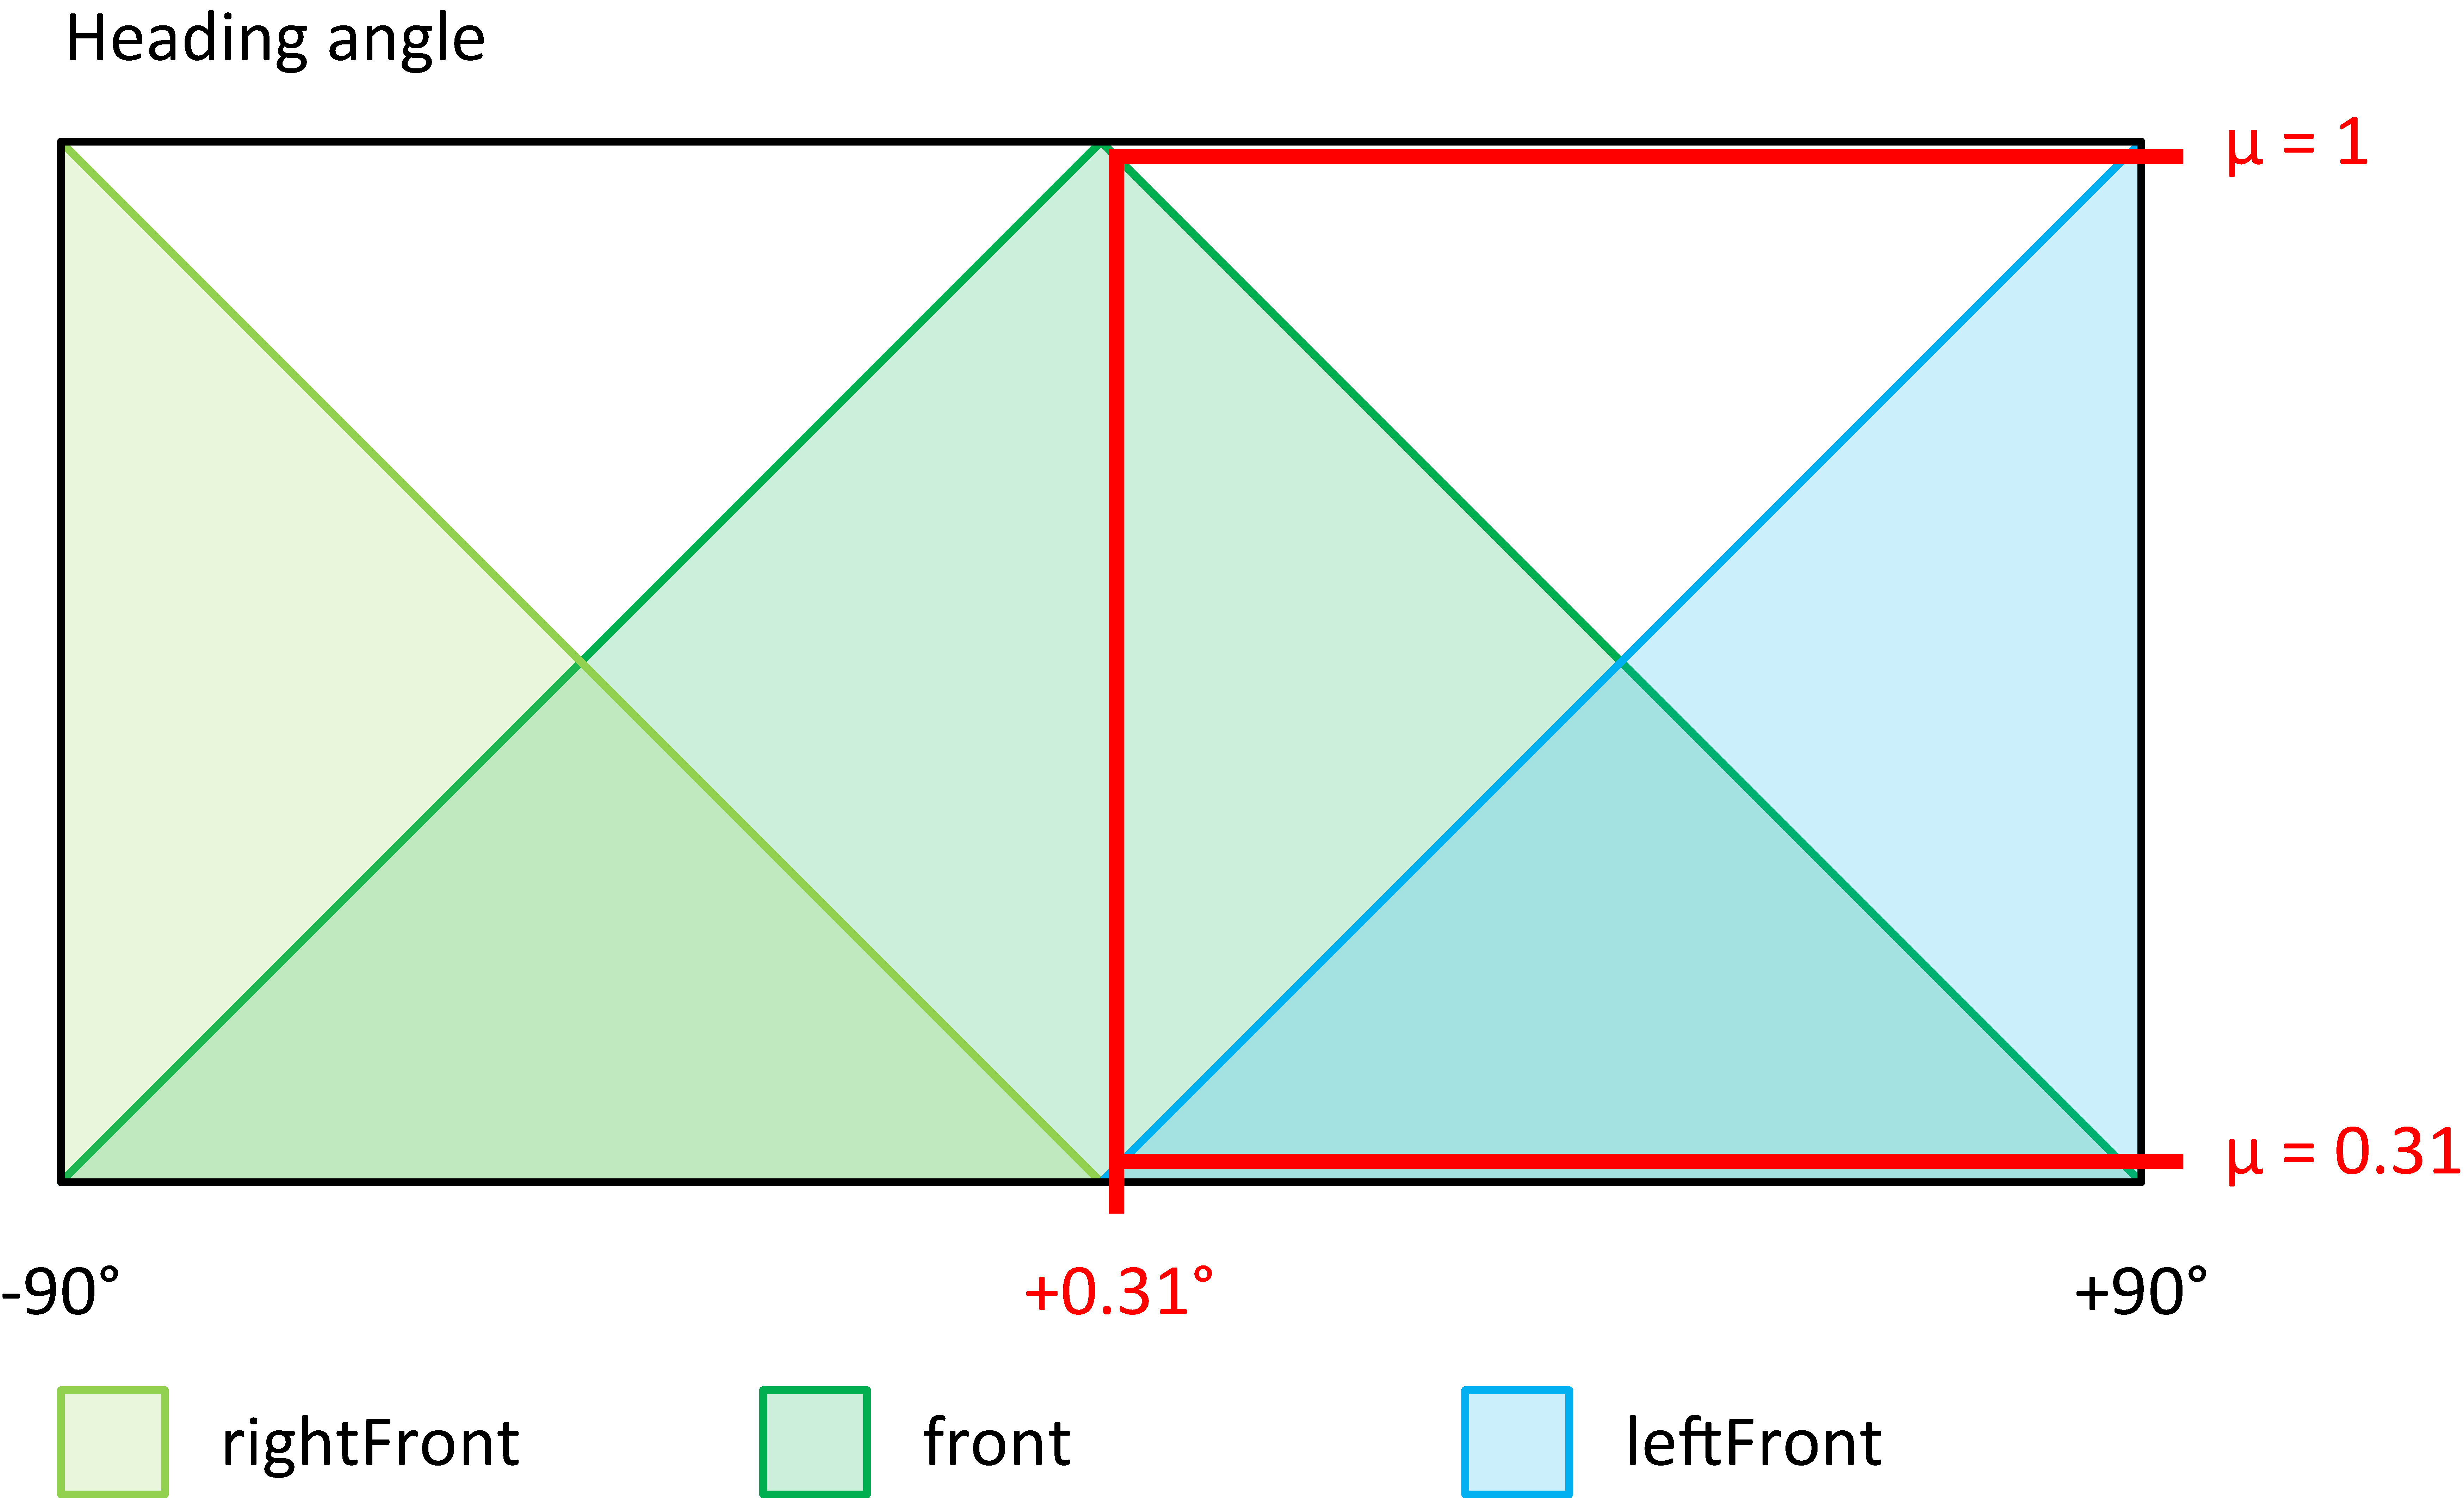
\includegraphics[scale=0.1]{./img/pdf/turnRule_headingAngle.pdf}
\end{figure}

Figure 6 shows a simplified view of the \emph{heading angle} sets, only displaying -90$^{\circ}$ to +90$^{\circ}$ during the firing of Rule 1 and Rule 2. The \emph{heading angle} value of +0.31$^{\circ}$ belongs to the \emph{front} fuzzy set at $\mu$ = 1, and also belongs to the \emph{leftFront} fuzzy set at $\mu$ = 0.31, hence the firing of the two rules, thus providing two inputs. These inputs, along with the \emph{energy difference} input will be aggregated to create a single, crisp output, as explained in the next section.

\subsubsection{Rule aggregation}

When multiple inputs are provided by the same linguistic variable antecedent, as seen in Section 4.1.2, Sugeno style inference calculates the weighted average to provide a single, crisp input, using the following formula:

{\LARGE
	\begin{align}
	\mbox{WA} = \frac{\sum^N_{i=1} \mu(k_i) k_i}{\sum^N_{i=1} k_i}
	\end{align}
}

\noindent
Therefore, to calculate the weighted average for the two \emph{heading angle} inputs for the example shown in Figure 6:

{\LARGE
	\begin{align}
	\mbox{WA} &= \frac{1 \times 0.31 + 0.31 \times 0.31}{1 + 0.31} \\
	&= 0.31
	\end{align}
}

\noindent
Subsequently, the crisp output from the two \emph{heading angle} antecedents is 0.31. However, $\mu$ for the \emph{energy difference} antecedent must also be considered. As discussed in Section 4.1.1, $\mu$ = 1 for \emph{energy difference}.

Since the example rule performs an AND operation between the two antecedents, fuzzy set operations dictate that an intersection operation must occur to determine the final, crisp output. Therefore, the following function is appropriate:

{\LARGE
	\begin{align}
	\mbox{output} = \mbox{min}(\mu(k_1), \mu(k_2), \mbox{...}, \mu(k_n))
	\end{align}
}

\noindent
When applied to our example rules that have been fired:

{\LARGE
	\begin{align}
	\mbox{output} &= \mbox{min}(1, 0.31) \\
	&= 0.31
	\end{align}
}

\noindent
Therefore, the final, crisp output for the example scenario is a turn of 0.31$^{\circ}$. In other words, from its current direction of 0.0$^{\circ}$, the saucer will turn LEFT for 0.31$^{\circ}$, in order to follow the enemy, who is in front, and slightly to the left.